\documentclass[tikz]{standalone}
\usepackage{booktabs}
\usepackage{tikz}

\usetikzlibrary{arrows,automata,shapes}
%  \tikzset{
% Hypervisor/.style = {draw, minimum width=5cm},
% page/.style= {rectangle , draw = black, thick, minimum width = 1cm,minimum height =0.5 cm},
% VM/.style = { rectangle, draw=black!80, thick,minimum width=2cm,minimum height=1.2cm}}


\begin{document}
\begin{figure}[!h]
\centering
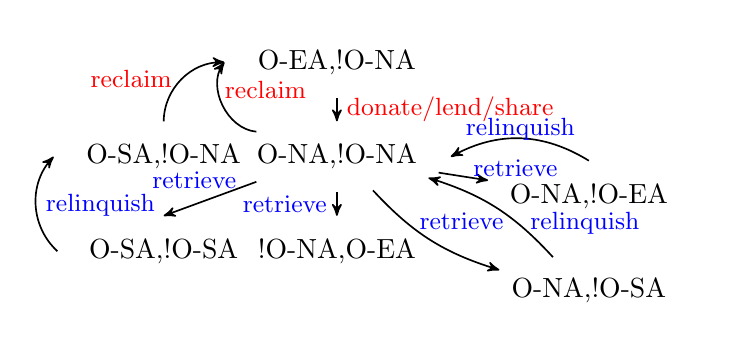
\begin{tikzpicture}[->,>=stealth',auto,node distance=1.2cm, semithick]
  \tikzstyle{every state}=[ellipse,draw=none,text=black,scale =1,inner sep=0pt]

  \node[state] (A)                    {O-EA,!O-NA};
  \node[state] (B) [below of= A]      {O-NA,!O-NA};
  \node[state] (C1) [below of= B]      {!O-NA,O-EA};
  \node[state] (C2) [left of= C1,xshift=-1cm]      {O-SA,!O-SA};
  \node[state] (C3) [right of= B,xshift=2cm,yshift=-0.5cm]      {O-NA,!O-EA};
  \node[state] (C4) [below of= C3]      {O-NA,!O-SA};
\node[state] (B2) [left of= B,xshift=-1cm]      {O-SA,!O-NA};

  \path (A.south) edge node[color=red] {\small donate/lend/share} (B.north)
  (B.south) edge node[color=blue,left] {\small retrieve} (C1.north)
  (B.south west) edge node[color=blue,above,xshift=-0.2cm] {\small retrieve} (C2.north)
  (B) edge[bend right = 0] node[color=blue,right,yshift=0.1cm] {\small retrieve} (C3)
  (C3.north) edge[bend right] node[color=blue,above,yshift=-0.15cm] {\small relinquish} (B.east)
  (B) edge[bend right=15] node[color=blue,above,xshift=0.4cm,yshift=0cm] {\small retrieve} (C4)
  (C2.west) edge[bend left=45] node[color=blue,right,xshift=0cm] {\small relinquish} (B2.west)
  (B2.north) edge[bend left=45] node[color=red,left,xshift=0cm] {\small reclaim} (A.west)
  (B.north west) edge[bend left=60] node[color=red,right,xshift=-0.1cm,yshift=0.2cm] {\small reclaim} (A.west)
  (C4) edge[bend right=15] node[color=blue,right,xshift=0.3cm,yshift=-0.2cm] {\small relinquish} (B)
  ;
        % (B) edge [loop above] node {1,1,L} (B)
        %     edge              node {0,1,L} (C)
        % (C) edge              node {0,1,L} (D)
        %     edge [bend left]  node {1,0,R} (E)
        % (D) edge [loop below] node {1,1,R} (D)
        %     edge              node {0,1,R} (A)
        % (E) edge [bend left]  node {1,0,R} (A);
\end{tikzpicture}
  \end{figure}


\end{document}
